\documentclass[conference]{IEEEtran}
\IEEEoverridecommandlockouts
% The preceding line is only needed to identify funding in the first footnote. If that is unneeded, please comment it out.
\usepackage{cite}
\usepackage{amsmath,amssymb,amsfonts}
\usepackage{algorithmic}
\usepackage{graphicx}
\usepackage{textcomp}
\usepackage{xcolor}
\graphicspath{{resources/}}
\def\BibTeX{{\rm B\kern-.05em{\sc i\kern-.025em b}\kern-.08em
    T\kern-.1667em\lower.7ex\hbox{E}\kern-.125emX}}
\begin{document}

\title{Development of Code Execution Visualization as Interactive Learning Tool for Online Programming Learning Platform}

\author{
  \IEEEauthorblockN{Faris Rizki Ekananda}
  \IEEEauthorblockA{\textit{School of Electrical Engineering and Informatics} \\
    Institut Teknologi Bandung\\
    Bandung, Indonesia \\
    faris.ekananda20@gmail.com}
  \and
  \IEEEauthorblockN{Yudistira Asnar}
  \IEEEauthorblockA{\textit{School of Electrical Engineering and Informatics} \\
    Institut Teknologi Bandung\\
    Bandung, Indonesia \\
    yudis@itb.ac.id}
}

\maketitle

\begin{abstract}
  One of the challenges in learning programming for people who are new to programming is understanding how programs work. This is important because they still don't have an appropriate view of the program's working process, making it difficult for them to absorb the programming material they learn. This is made more difficult when learning is done online, because learning can take place asynchronously so that teachers must be able to ensure understanding can be achieved through learning materials without direct interaction.

  One way to improve understanding in learning is by creating an interactive learning environment (ILE). In some existing online programming learning platforms, interactive learning is done by working on problems using a Web IDE such as Sololearn, understanding concepts using interactive visual animations such as Brilliant, and presenting material using interactive storytelling on Progate. However, the use of visualization of the execution of the program as an ILE is still minimally used in programming learning classes, even though based on several literature studies it can improve the understanding of programming concepts because it can generate a concrete model of computer programming in novice students.

  In this paper, an ILE is built in the form of a code execution visualization tool that displays how the program works. This system is integrated with online programming classes on KodeBareng Web Platform so that it can be used in the learning process and practice problem solving. After conducting user experiments, the results show that this ILE is considered by users to be helpful in learning with an average score in the range of 4.231 and 4.385 on the likert scale, as well as increasing the average correct answer value on the questions tested with the most significant increase in concept understanding (using SOLO Level) in module 1 with a t value of 2.179 (\textit{p = 0.0147}) for students who have never learned programming before with an increase from an average SOLO Level score of 2.429 to 3.857 and in module 2 from an average SOLO Level of 3.333 to 3.6.
\end{abstract}

\begin{IEEEkeywords}
  programming learning, interactive learning, code execution visualization
\end{IEEEkeywords}

\section{Introduction}
The rapid development of digital technology opens up vast potential in online learning. With the help of the internet, learning can be done anywhere and anytime. Learning is no longer constrained by geographical and time boundaries so that there are more connections and interactions between teachers and students \cite{choy2004interactive,keengwe2010towards,psotka2012ile}.

However, the interaction between students and teachers in online learning cannot be equated with traditional learning. Interactions such as verbally asking students questions, encouraging students to solve problems in front of the class, and similar things cannot be done in asynchronous online learning because the interaction between the student and the teacher is not done directly.

One of the challenges experienced by people who are new to programming is the lack of understanding of what happens when a program executes a code \cite{mayer1981psychology, moons2013pilot}. This happens because they still don't have a proper idea of how a computer program works, which makes it difficult for them to grasp the fundamental and abstract concepts of learning programming for beginners. Online learning also makes this more difficult to overcome as there is less interaction between the student and the teacher during asynchronous learning, so the teacher has to use other tools to provide a concrete model to the student.

Currently, many programming learning platforms utilize interactive learning in the form of code exercises using Web IDEs, interactive visual animations, and interactive storytelling. However, these solutions cannot address the problems faced by students who have never learned programming before. An interactive environment that supports learning and practicing programming tasks is needed to solve these problems. Such a environment is aimed to improve concept understanding, make learning more interactive and facilitate the students during the learning process.

In this paper, we will focus on the development of a code execution visualization tool as an interactive learning environment that can support the conceptual understanding of how a program works for students who are new to programming. We will also observe the effect of the tool on the learning process of students.

\section{Literature Review}
\subsection{Interactive Learning}
Essentially, interactive learning is a method of learning that involves interaction between the student and the educational material, such as processing the material, completing tasks, or solving problems with the aim of building cognitive, affective, conative, and psychomotor learning outcomes. In short, there is a reciprocal action relationship between student and teacher which prevents learning from becoming passive. In the context of online learning, this can be achieved through digital technology that connects students and teachers.

The characteristics of interactive learning \cite{reeves2012interactive} are access to content, tasks, and problems by the students using digital technology such as computers with internet access. Furthermore, Reeves \cite{reeves2012interactive} explains that there are 2 approaches in the application of interactive learning, namely learning "through" interactive learning program and learning "with" interactive learning program. Learning "through" an interactive learning program means that the program provides the lesson in a variety of communication methods (focusing on the interactive delivery of the lesson) while learning "with" an interactive learning program utilizes cognitive tools that the student can use to build pieces of information into knowledge allowing the student to build their own familiar representational model of understanding. Learning "with" an interactive learning program is much more impactful as it facilitates critical thinking and higher-order thinking (HOT). The program or tool used in interactive learning is also referred to as an interactive learning environment (ILE).

\subsection{Interactive Learning Environment (ILE)}
There are various types of interactive learning environments that can support learning programming according to \cite{moons2013pilot}, such as \textit{microworlds} that use graphics like LOGO turtles or in the form of physical robots such as Lego Mindstorm Kit that use simplified programming languages, algorithm visualization tools to visualize the workflow of a specific algorithm, and code execution visualization tools that can display the flow of a program's work process when executed. Sites that offer online learning, such as \cite{sololearn2021media}, \cite{codesaya2021media}, \cite{brilliant2021media}, and learning portals of educational institutions or \textit{e-learning system} are also considered as ILEs using the first form of interactive learning approach which is " through" interactive learning because it is static.

One form of ILE used in learning programming is a web-based integrated development environment (IDE) (hereafter referred to as Web IDE), which allows programming learners to write code and run it. This is because Web IDEs allow users to directly implement code without having to do any setup first. The Web IDE can also ensure that the program execution environment will always be the same between one user and another, and increase portability because it can be done anytime and anywhere \cite{tran2013interactive}. These ILEs can be integrated with program execution visualization tools so as to improve learners' understanding of programming concepts \cite{moons2013pilot}. Such ILEs fall under the second interactive learning approach of "with" interactive learning as they provide tools that users can use to explore further. Examples of ILEs in the form of code execution visualizations can be seen in Fig.~\ref{fig:pythontutor} and Fig.~\ref{fig:evizor}

\begin{figure}[htbp]
  \centerline{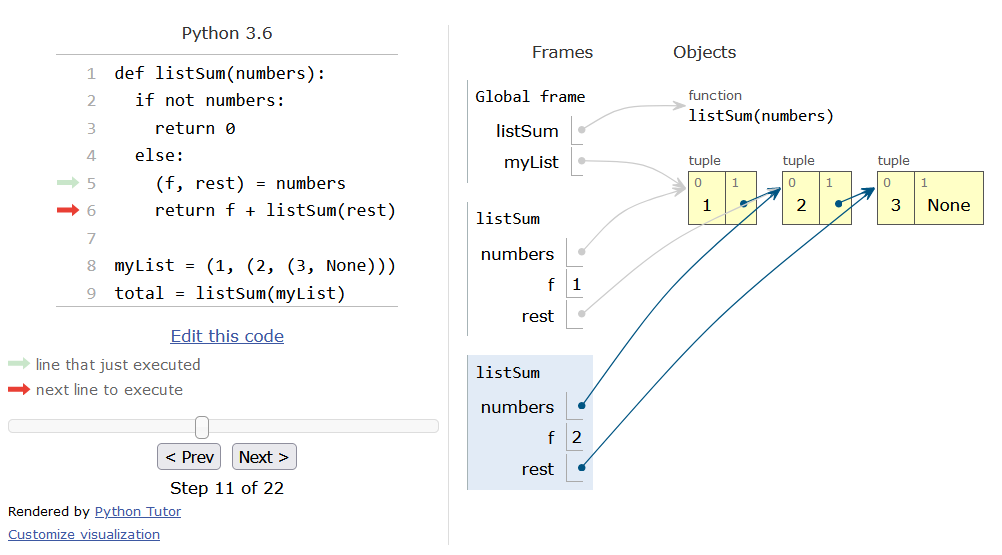
\includegraphics[width=\linewidth]{chapter2/pythontutor.png}}
  \caption{Code Execution Visualization in Python Tutor} \label{fig:pythontutor}
\end{figure}

\begin{figure}[htbp]
  \centerline{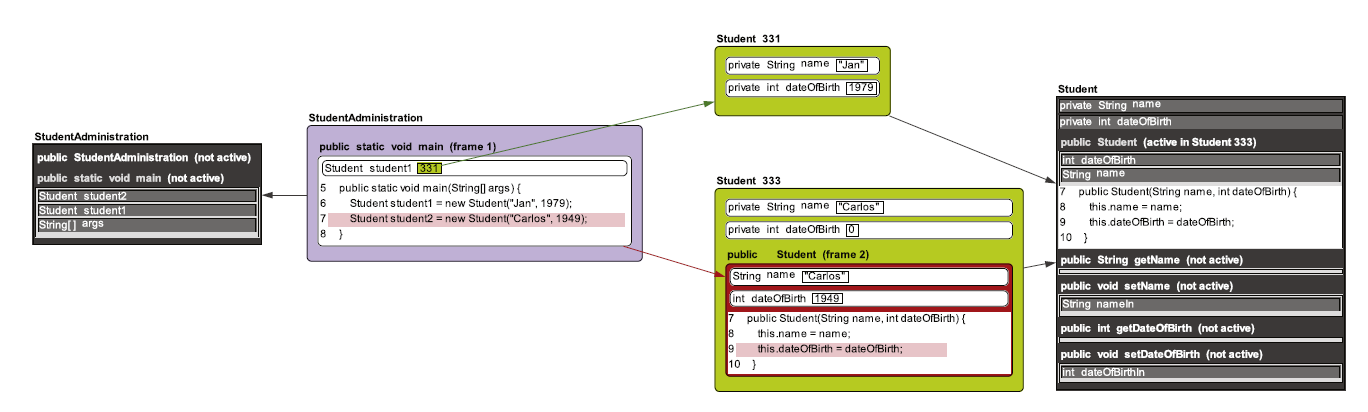
\includegraphics[width=\linewidth]{chapter2/evizor.png}}
  \caption{Code Execution Visualization in EVIZOR} \label{fig:evizor}
\end{figure}

\section{Related Works}
From several learning class platforms, online interactive programming learning methods can be categorized into visual and non-visual. Visual programming learning methods do not directly use code as in \cite{brilliant2021media}, but use interactive visual analogies using images, symbols, and animations. This method makes learning more interesting and easier because it is expressed in visual form so that it can model the learner's frame of mind. However, this method does not directly touch on practical programming activities, so there may be a discrepancy between the theory and practice understood by the students and the actual implementation of the program. This method is also content-specific, so it cannot be used for other content. \cite{froggy2021media} is also included in this category, because its implementation is only specific to the material covered, especially in web development materials.

\begin{figure}[htbp]
  \centerline{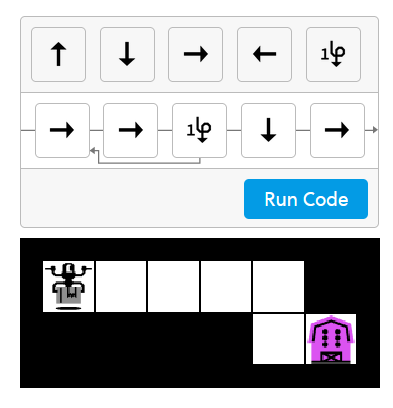
\includegraphics[width=0.4\linewidth]{chapter2/brilliant.png}}
  \caption{\label{fig:brilliant}One of interactive learning example in Brilliant}
\end{figure}

Non-visual methods mostly use Web IDEs in their learning. Students can interact with the Web IDE so that they can practice practical problem-solving and programming skills. The Web IDEs used usually have the capability to return the output of the code execution, as well as to assess the correctness of the implementation, as seen in \cite{sololearn2021media}. Web IDEs can also accept various languages according to the needs of the material being studied. In addition, there are also Web IDEs that simulate a terminal rather than a code editor as can be seen in Katacoda \cite{katacoda2021media}. There are also platforms such as \cite{progate2021media} that utilize interactive learning with a "through" approach of delivering material visually and narratively. However, most of the implementations of these methods only focus on the practical programming exercises aspect, not paying attention to the student issues previously discussed.

\begin{figure}[htbp]
  \centerline{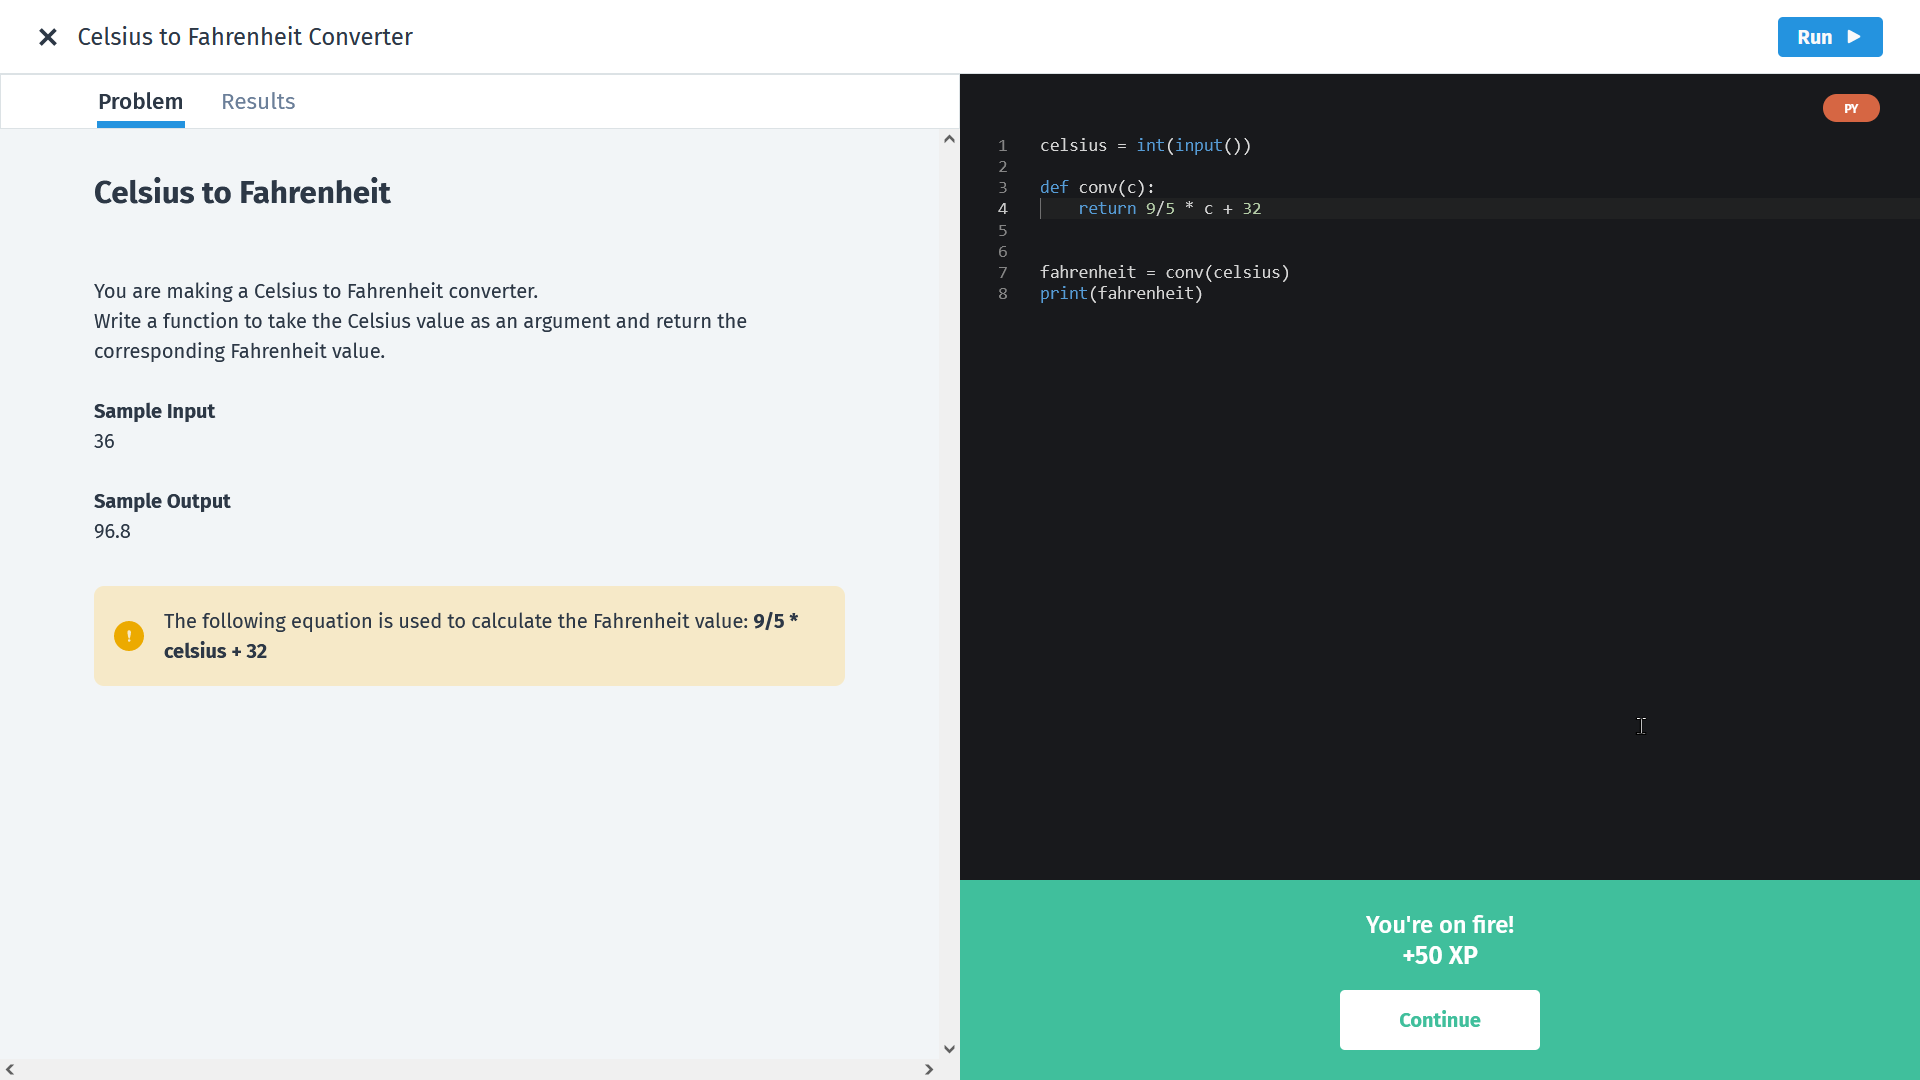
\includegraphics[width=\linewidth]{chapter2/sololearn.png}}
  \caption{\label{fig:sololearn}Code practices in Sololearn}
\end{figure}

\section{Analysis and Design}
\subsection{Problem Approaches}
The complexity of programming itself makes it difficult for students who are new to programming to understand the concepts and abstracts of programming \cite{moons2013pilot}. The lack of ability to trace the traces of a program code, as well as the unformed framework model of how computer programs work \cite{mayer1981psychology} are factors that make students unable to absorb new technical information related to programming to the fullest. Therefore, a concrete model is needed related to the workflow of a computer program so that it can facilitate the process of transferring knowledge of programming concepts to students. Interactive learning is one way that can be utilized because it can be applied online using digital technology that is already available.

According to \cite{moons2013pilot}, there are 4 approaches that can be taken to solve the problem. The first approach is to use a certain sequence of programming paradigms in learning such that deeper concepts in programming do not have to be learned from the beginning. The second approach is to use active learning techniques, such as workshops and narrative storytelling. However, this approach is rather difficult to apply to online learning. The third approach is to use programming languages that are more suitable for programming students, such as Python and Eiffel. The fourth approach is to use an interactive learning environment (ILE) that can be in the form of a microworld, algorithm visualization, and code execution visualization.

\subsection{Code Execution Visualization}
ILEs in the form of code execution visualization tools can also be used to implant a concrete model of a framework for thinking about how computers work \cite{mayer1981psychology} and can also help students in tracing the workflow of computer programs. With code execution visualization, students can explore the ILE so as to build an understanding of the concept of program work with their own thinking and make interactive learning using the second approach of learning "with" interactive learning which is more effective \cite{reeves2012interactive}. Code execution visualization can also improve the support for practical programming activities, thus improving the support for online programming learning. Code execution visualization can be integrated in the learning material module according to the suggestion of the locus of providing concrete models according to \cite{mayer1981psychology} as well as in programming exercises as in research \cite{moons2013pilot}

\subsection{Functional Requirement}
In developing the ILE in the form of code execution visualization, a use case diagram is designed according to the needs and related approaches that can be seen in Fig.~\ref{fig:diagram-usecase-paper}.

\begin{figure}[htbp]
  \centerline{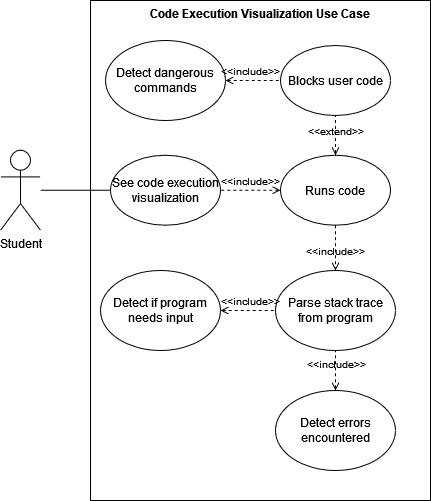
\includegraphics[width=0.7\linewidth]{chapter3/diagram_usecase_paper.jpg}}
  \caption{\label{fig:diagram-usecase-paper}Use Case Diagram}
\end{figure}

Based on the use case diagram that have been created in Fig.~\ref{fig:diagram-usecase-paper}, functional and non-functional requirements are derived which can be seen in Table~\ref{tab:srs-fungsional} and Table~\ref{tab:srs-nonfungsional}.

Functional requirements describe the functions that can be performed on the ILE to be created. These requirements are derived from the use case diagram according to who and what can be done. A more detailed explanation of functional requirements can be seen in Table~\ref{tab:srs-fungsional}.

\begin{table}[htbp]
  \caption{Functional Requirement}
  \begin{center}
    \begin{tabular}{|l|p{0.3\linewidth}|p{0.4\linewidth}|}
      \hline
      \textbf{ID} & \textbf{Requirement}                                  & \textbf{Description}                                                                                 \\ \hline
      KB-F-01     & User enters program code on the system                & -                                                                                                    \\ \hline
      KB-F-02     & User enters input for the program on the system       & Input is asked if the program needs input                                                            \\ \hline
      KB-F-03     & User runs the code                                    & User can see the output of the program                                                               \\ \hline
      KB-F-04     & User can see code execution visualization             & User can see the change in data and flow of the program                                              \\ \hline
      KB-F-05     & User can see error messages from the program          & -                                                                                                    \\ \hline
      KB-F-06     & System blocks user code if it contains dangerous code & -                                                                                                    \\ \hline
      KB-F-07     & System process program stack trace for visualization  & Stack trace includes variables, functions, modules, and stack frames. Python debugger (pdb) is used. \\ \hline
    \end{tabular}
    \label{tab:srs-fungsional}
  \end{center}
\end{table}

\subsection{Nonfunctional Requirement}
Nonfunctional requirements are derived so that the objectives can be achieved and the system runs smoothly. Therefore, requirements are derived in the form of limitations on the response of execution results so that students do not wait too long for the results of execution, system design that makes it easy to test various kinds of code, and limit what can be executed so that system security can be maintained. A more detailed explanation of the nonfunctional requirements can be seen in Table~\ref{tab:srs-nonfungsional}.

\begin{table}[htbp]
  \caption{Nonfunctional Requirement}
  \begin{center}
    \begin{tabular}{|l|l|p{0.4\linewidth}|}
      \hline
      \textbf{ID} & \textbf{Parameter} & \textbf{Requirement}                                              \\ \hline
      KB-NF-01    & Performance        & The system returns the execution result within 10 seconds at most \\ \hline
      KB-NF-02    & Testability        & The system is easy to test                                        \\ \hline
      KB-NF-03    & Security           & The system does not allow malicious code execution                \\ \hline
    \end{tabular}
    \label{tab:srs-nonfungsional}
  \end{center}
\end{table}

\subsection{Component Diagram}
Based on the results of the previous problem and needs analysis, the design of the implementation components was made. The design is in the form of a component diagram found in Fig.~\ref{fig:diagram-komponen}. This design illustrates what components will be added to the system if the ILE needs to be integrated to existing programming learning platform.
\begin{figure}[htbp]
  \centerline{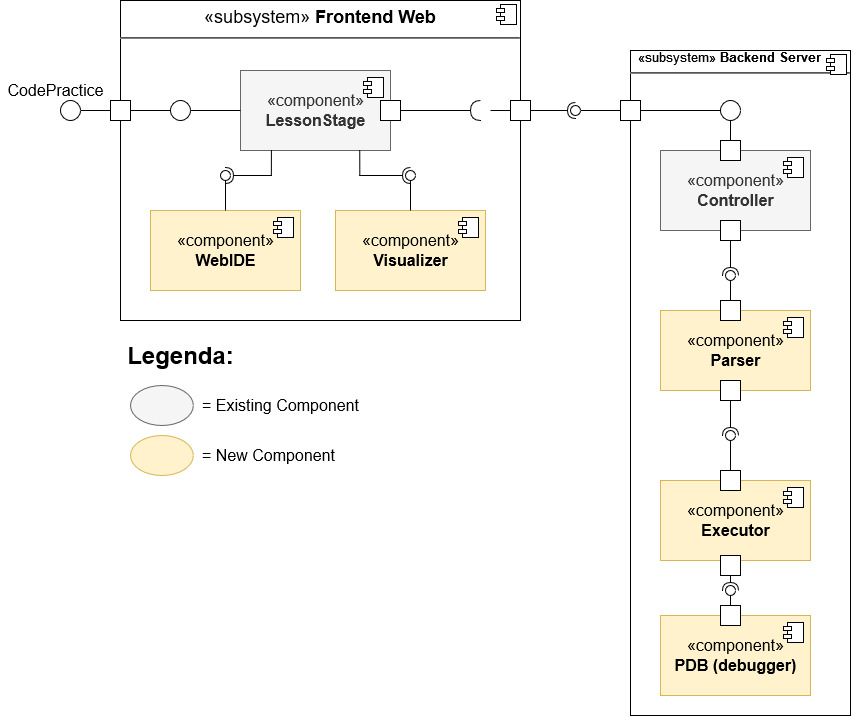
\includegraphics[width=0.8\linewidth]{chapter3/diagram_komponen_paper.jpg}}
  \caption{Component Diagram} \label{fig:diagram-komponen}
\end{figure}

\subsection{Visualizer}
In the Frontend system, a new component is added, namely the Visualizer, which can visualize the execution code entered in the Web IDE component. The Visualizer must be able to display the contents of a program as it runs at each step of its execution, such as the lines of code being executed, the contents of the variables contained in the program's memory, the program's output, and any error messages that occur. Visualizer can be explored by the user by changing the input entered in the executed program, changing the program code that you want to visualize, and can see the flow of program code execution forward or backward that can be controlled by the user.

\subsection{Stack Trace Processing}
In the Backend system, new components are created to get the information needed for visualization. The \verb|PDB (debugger)| component is a built-in \verb|Python| component that can be used for debugging code. The \verb|Executor| component is used to execute program code using PDB so that it can automatically explore the execution of program code and get a stack trace. The \verb|Parser| component is used to process the execution results and stack trace from \verb|Executor| so that it can be used for visualization of code execution. The workflow design of the Executor and Parser components can be seen in Fig.~\ref{fig:activity-executor}

\begin{figure}[htbp]
  \centerline{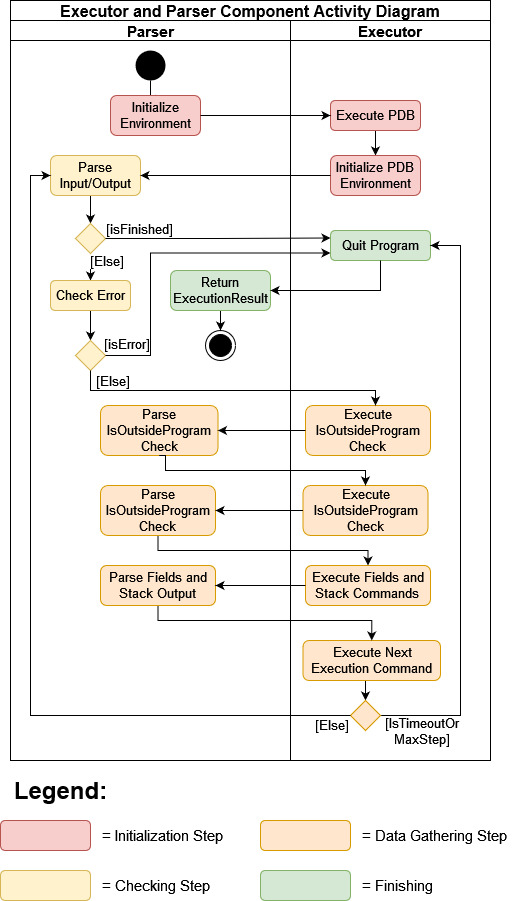
\includegraphics[width=0.6\linewidth]{chapter3/activity-executor-paper.jpg}}
  \caption{Executor and Parser Component Activity Diagram} \label{fig:activity-executor}
\end{figure}

\section{Implementation and Testing}
\subsection{Environment and Tools}
Development is done using computer that has Ubuntu 20.04 LTS operating system, 2GB of memory, 32GB of storage, and 1 core Intel(R) Xeon(R) CPU E5-2660 0 @ 2.20GHz. This computer is a server that is connected to the internet which also used for Backend system.
The Frontend system is developed with Nuxtjs and deployed on Cloudflare Pages. The Backend system is developed in Nodejs environment with Expressjs and Docker, and is deployed on the server.

\subsection{Limitation}
Programming language that needs to be visualized is limited to Python 3.9. The application produced is also limited in the form of minimum viable product (MVP). MVP is a product that only suffice its features based on user needs without further sophistication. The purpose of MVP is to get feedback and attract potential users.

\subsection{Implementation}
\paragraph{Executor Component}
The Executor component is a component used to execute program code using PDB. This component requires input in the form of a file location containing the program code to be executed and the input to be given to the program. There are 3 main stages in this component, namely the initialization stage, the checking stage, and the data collection stage. An illustration of the Executor workflow can be seen in Fig.~\ref{fig:activity-executor}
\paragraph{Parser Component}
The Parser component is a component used to process the output of the Executor component. This component also determines the logic and steps to be taken by the Executor Component. This component requires input in the form of \verb|array of strings| which is the output of the Executor Component which has been separated per line. There are 2 main stages in this component, namely the checking stage and the data collection stage. An illustration of the Parser workflow can be seen in Fig.~\ref{fig:activity-executor}

\subsection{Alpha Testing}
Functional testing was conducted based on the ILE functional and nonfunctional requirement in Table~\ref{tab:srs-fungsional} and Table~\ref{tab:srs-nonfungsional}. Test scenarios and results can be found in Table~\ref{tab:fungsional-testing} and Table~\ref{tab:nonfungsional-testing}.
\begin{table}[htbp]
  \caption{Functional Requirement Testing}
  \begin{center}
    \begin{tabular}{|l|p{0.5\linewidth}|l|}
      \hline
      \textbf{ID} & \textbf{Requirement}                                  & \textbf{Result} \\ \hline
      KB-F-01     & User enters program code on the system                & Success         \\ \hline
      KB-F-02     & User enters input for the program on the system       & Success         \\ \hline
      KB-F-03     & User runs the code                                    & Success         \\ \hline
      KB-F-04     & User can see code execution visualization             & Success         \\ \hline
      KB-F-05     & User can see error messages from the program          & Success         \\ \hline
      KB-F-06     & System blocks user code if it contains dangerous code & Success         \\ \hline
      KB-F-07     & System process program stack trace for visualization  & Success         \\ \hline
    \end{tabular}
    \label{tab:fungsional-testing}
  \end{center}
\end{table}
\begin{table}[htbp]
  \caption{Nonfunctional Requirement Testing}
  \begin{center}
    \begin{tabular}{|l|l|l|}
      \hline
      \textbf{ID} & \textbf{Parameter} & \textbf{Result} \\ \hline
      KB-NF-01    & Performance        & Success         \\ \hline
      KB-NF-02    & Testability        & Success         \\ \hline
      KB-NF-03    & Security           & Success         \\ \hline
    \end{tabular}
    \label{tab:nonfungsional-testing}
  \end{center}
\end{table}
\subsection{User Experiment}
An experiment was designed that would measure students performance on a introduction learning module related to the understanding of basic programming concept such as input/output, data types and conversion, and expression operation. The goal of the experiment is to measure the students' ability to understand the basic programming concept. Experiment is conducted in KodeBareng, which is an online programming learning platform that has been integrated with the code execution visualization ILE.

Of the 42 people who signed up for the experiment through the form, 25 responded and were able to schedule the experiment and thus became legitimate experiment participants. Then, participants were mapped into a 13-person treatment group and a 12-person control group.

The experiment was conducted online using the Google Meet platform. Participants were provided with the Google Meet link according to the predetermined experiment cluster schedule. Participants were asked to use a laptop/computer while conducting the experiment. After all participants in a cluster have entered into Google Meet, participants are given a link to the questionnaire form to fill in their identity first. Then, participants were directed to the KodeBareng website, created a KodeBareng account using a Google account, and then opened the class according to their respective groups. Before starting learning, participants were given directions on how to learn at KodeBareng and instructions to do learning at their own pace for 1 hour. Especially for participants in the treatment group, they were given an introduction to how to use the ILE that had been provided during the learning. After 1 hour had passed, participants were asked to stop learning and continue filling out the questionnaire.
\subsection{Experiment Results}
From the test analysis results with 13 treatment group participants and 12 control group participants (a total of 25 participants obtained by convenience sampling), participants in the treatment group felt the positive impact of the ILE with a score of 4.231 on the criteria for understanding the code run and a score of 4.385 on the criteria for helping to answer quizzes and practice questions as seen in Fig.~\ref{fig:kuesioner-average-paper}.
\begin{figure}[htbp]
  \centerline{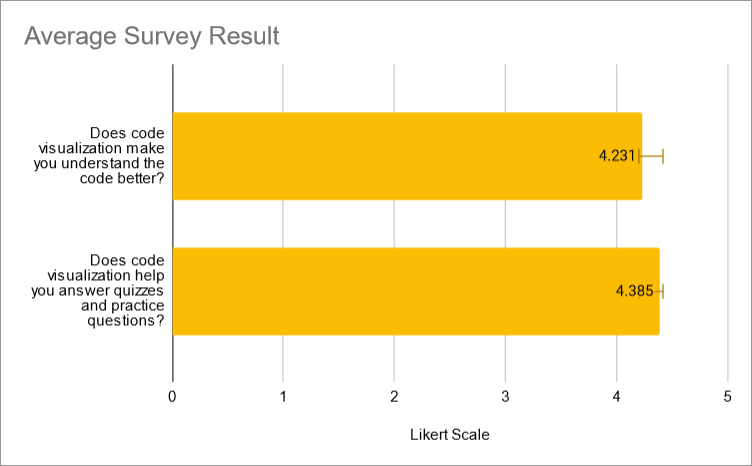
\includegraphics[width=0.6\linewidth]{chapter4/kuesioner-average-paper.png}}
  \caption{Survey Results} \label{fig:kuesioner-average-paper}
\end{figure}

In addition, there was a consistent increase in the average percentage of quizzes with correct answers as seen in Fig.~\ref{fig:eksperimen-k1k2-kebenaran-awam-paper},
\begin{figure}[htbp]
  \centerline{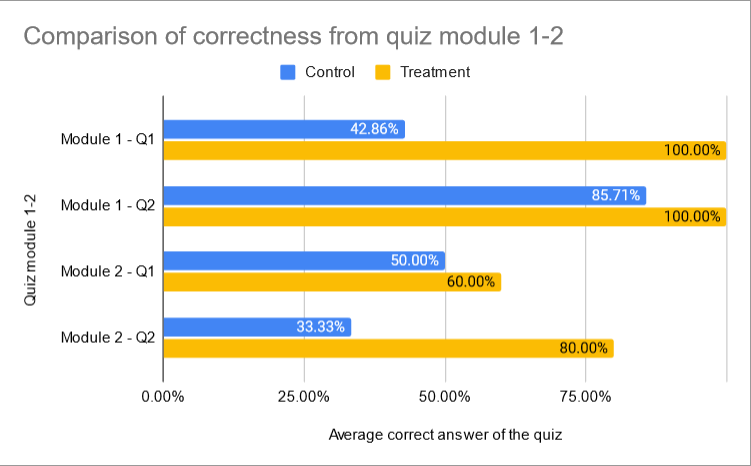
\includegraphics[width=0.6\linewidth]{chapter4/eksperimen-k1k2-kebenaran-awam-paper.png}}
  \caption{Average Quiz Correctness} \label{fig:eksperimen-k1k2-kebenaran-awam-paper}
\end{figure}
as well as an increase in the average understanding of concepts in the code exercise questions (as seen in Fig.~\ref{fig:eksperimen-lk1-awam-paper}) with the most significant result in module 1 with a t-value of 2.179 (\textit{p = 0.0147}) with an increase from an average of 2.429 in the control group to 3.857 average in the treatment group as well as in module 2 with an increase from 3.333 average in the control group to 3.6 average in the treatment group but with a t-value of 2.262 (\textit{p = 0.662}) which was not significant due to fewer experimental participants who could complete the second module than the first module.
\begin{figure}[htbp]
  \centerline{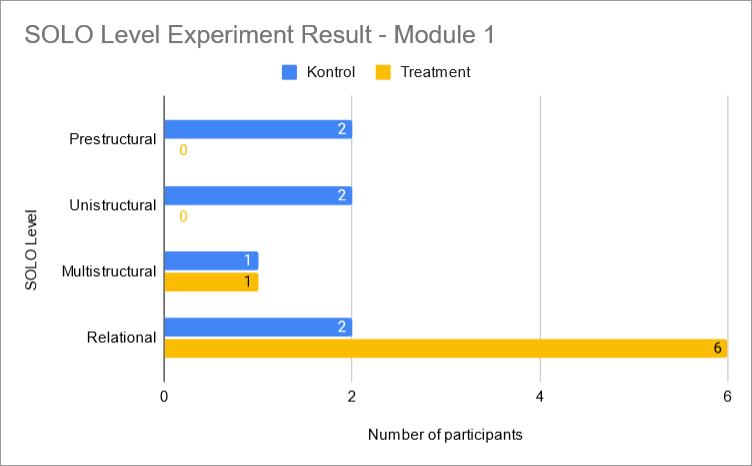
\includegraphics[width=0.6\linewidth]{chapter4/eksperimen-lk1-awam-paper.png}}
  \caption{SOLO Level Comparison} \label{fig:eksperimen-lk1-awam-paper}
\end{figure}
Furthermore, it was also found that another impact of ILE was to create distraction during the learning process, thus making the learning time longer as seen in Fig.~\ref{fig:eksperimen-m1m2-waktu-paper}.
\begin{figure}[htbp]
  \centerline{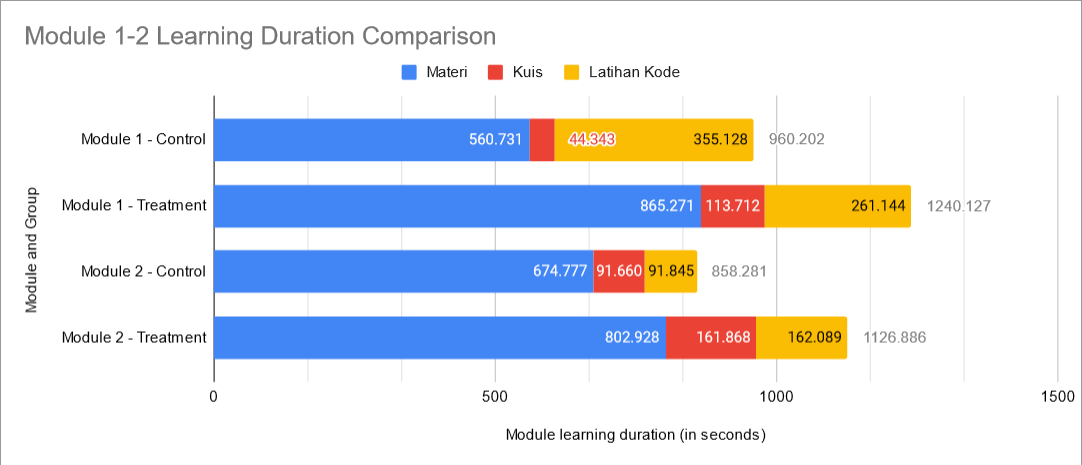
\includegraphics[width=0.6\linewidth]{chapter4/eksperimen-m1m2-waktu-paper.png}}
  \caption{Module Learning Duration Comparison} \label{fig:eksperimen-m1m2-waktu-paper}
\end{figure}

\section{Conclusion and Future Work}
ILE is proven to improve students' learning experience, and can improve the understanding of programming concepts and the workflow of a program for people who have never learned programming before.

The suggestions for future works related to the topics in this paper are as follows:
\begin{enumerate}
  \item ILE can be further developed using other interaction schemes, such as the use of animation in displaying visualizations, or other visual elements.
  \item A number of experiment participants experienced difficulties in interacting and navigating the ILE, so it can be an improvement point for further development.
  \item Support for more complete Python programming language features as well as support for other programming languages. The addition of this support allows the developed ILE to be used in more complex learning classes.
  \item There needs to be a study of the implementation of ILE in other approaches as mentioned by \cite{moons2013pilot} so that its effectiveness can be compared with the approach chosen in this Final Project.
  \item Testing with more academically appropriate learning materials and practice questions is needed to obtain more accurate experimental results. In addition, more experimental participants and sampling methods that are more representative of the entire population can also improve the accuracy of test results.
\end{enumerate}

\bibliographystyle{IEEEtran}
\bibliography{IEEEabrv,IEEE}

\vspace{12pt}

\end{document}
